\documentclass[a4paper,10pt]{article}
\usepackage[utf8]{inputenc}
\usepackage{graphicx}
\usepackage{amsmath}
\usepackage{amsfonts}
\usepackage{amssymb}
\usepackage{verbatim}
\usepackage{bm}
\usepackage{amsthm}
\usepackage{quoting}
\quotingsetup{font=small}
\usepackage[english]{babel}
\usepackage[toc,page]{appendix}
\usepackage[T1]{fontenc}
\usepackage{graphicx}
\usepackage{blindtext}
\usepackage{bm}
\usepackage{amsthm}
\usepackage{subfig}
\usepackage{tabularx}
\usepackage{amsbsy}
\usepackage{authblk}
\usepackage{lipsum} % for filler text
\usepackage{fancyhdr}
\usepackage{rotating}
\usepackage[section]{placeins}
\usepackage{booktabs}
\usepackage{caption}
\usepackage{tabularx}
\usepackage{setspace}
\usepackage{multicol}
\usepackage{amsbsy}
\usepackage{graphicx}
\usepackage{bm}
\usepackage{tabularx}
\usepackage{booktabs}
\usepackage{xcolor}
\usepackage{emptypage}
\usepackage[a4paper,top=4cm,bottom=3.5cm,left=3.4cm,right=3.4cm]{geometry}
\usepackage{csquotes}
\usepackage[maxbibnames=99,backend=biber]{biblatex}
\addbibresource{citazioni-OC-CML.bib}
\nocite{*}
\input{epsf}
\def\hbn{{\hfill\break\noindent}}
\DeclareMathOperator{\sgn}{sgn}
\DeclareMathOperator{\Ree}{Re}
\DeclareMathOperator{\Imm}{Im}
\DeclareMathOperator{\Minn}{Min}
\DeclareMathOperator{\Maxx}{Max}
\DeclareMathOperator{\Supp}{sup}
\date{}
\author{}
\begin{document}
\title{Optimization of Imatinib chronic myeloid leukemia's therapy via control theory}
\maketitle



\section{Introduction}
The chronic myeloid leukemia (CML) is a clonal myeloproliferative  human blood cancer that 
makes up approximately 15\% of all leukemias in adults (cit).
Different mathematical models were developed to study
hematopoiesis, this is caused by the relative facility of sampling blood or bone marrow.\\
Some examples of this mathematical models are
 a discrete collection of ordinary differential equations,
 each of which describes a
maturation stage  of the cells \cite{michor2005, sottoriva, czochra}.
 Another group of models  takes in account the 
stochasticity in the cell fate decision \cite{till1964stochastic,tomasetti2010role}.\\
Mathematical hierarchically models for the CML have proved useful for deriving prognostic
informations the course of the disease 
and the parameters that describe the mechanism of the
pathology
\cite{michor2005, sottoriva, olshen2014dynamics, tang2011dynamics}.

In this work we will consider a simple example of hierarchical 
model for leukemia  \cite{stiehl2012mathematical},  first we will
study the equilibrium of the model in order to classify the patients in function of their
parameters, and this will give to us the possibility to forecast the outcome of the therapy.\\
Then, since for this cancer exits a 
molecular target therapy (the tyrosine kinase inhibitor)
that gives a dramatic improvement of the clinical
situation of the patients; we will focus our attention 
about the optimization of the therapy,
since therapy has different drawbacks, for example is not clear that
if the therapy
is able to completely eradicate the disease \cite{michor2005}
so could be consider a life-long therapy and 
it is very expensive \cite{experts2013price}, 
this cost is so high that could limitate
application of the therapy \cite{himmelstein2009medical,chen2017journey},
then a optimal therapy protocol would lower the prices of therapy and 
more patients will be able to afford it. The economic  factor is not the only 
 cost that is possible to consider when optimizing a protocol, for example we will also
 consider the toxicity, the possibility to develop a resistant mutation and the performance
 in reducing the tumor burden.\\
Then we will describe a mathematical framework to 
find the optimal protocol for any therapy where the mathematical model of the
tumor dynamics and the pharmacokinetics of the drugs are known,
 to do that we will use the control theory,   in particular we will 
consider a open loop optimization to solve the optimal control problem \cite{chapman-book}.
\section{The mathematical model}

\subsection{Cell lineages}
Many healthy tissues are characterized 
by a hierarchical organization, and this hierarchical organization could be treated as
an ordered sequence of discrete maturation states.  In various literatures,
simple mathematical models 
are used to exploit this assumption for the study of healthy hematopoietic \cite{czochra} and
the dynamics involving the number of the cancer cells in a patient
\cite{sottoriva, michor2005,altrock2015mathematics, stiehl2018mathematical, stiehl2012mathematical}.\\
These models are built in the following ways:
\cite{sottoriva, michor2005, tang2011dynamics, olshen2014dynamics, altrock2015mathematics, stiehl2018mathematical, stiehl2012mathematical} 
we divide the cells of the tissue under the study in $n_{e}$ 
in non-intersecting ensembles, with every ensemble 
representing a certain stage of cell differentiation.
The time order of the differentiation stage defines a hierarchy of these ensembles.
We define a \textit{lineage} as a collection of ensembles that fully describe all
the stages of differentiation of cells within a certain tissue.\\ 
For every ensemble, we define a function
$c_{i,m}(t):\mathbb{R}\longrightarrow\mathbb{R}^+$ 
with $i=1,2,\dots,n_{e}$ and $m=1,2,\dots,m_{l}$.
These functions
represent the number of cells in the $i$ ensemble
in the $m$ lineage, at a time of $t$.
Firstly, we divide the hematopoietic system into three different ensembles:
\begin{enumerate}
\item Stem cells (SC),
\item Progenitor cells (PC),
\item Terminally differentiated (or post-mitotic/mature) cells (TD)
\end{enumerate}
a full model should 
consist of six different ensembles but, as stated, into
\cite{sottoriva, stiehl2012mathematical}. However,
this assumption does not improve  the agreement
analyzing clinical data.\\
The next step is to study the transition between ensembles,
since experimental data \cite{michor2005, tang2011dynamics, olshen2014dynamics, rainero2018gdna} 
show that the proliferation of healthy cells, along with the 
blast, and the decline under therapy of the BCR-ABL expression are exponential. 
This implies that the dynamics of the number of cells should be described
by first order differential equations
(or by a binomial process, if one wants to use probabilistic dynamics).\\
We thus focus our attention on the fluxes
between ensembles. Given the following constants:
\begin{itemize}
\item $p_{i,k}$ is the division rate of the cells in the $i$ ensemble of the $k$ lineage.
\item $d_{i,k}$ is the death rate of the cells in the $i$ ensemble of the $k$ lineage.
\item $a_{i,k}\in [0,1]$.
This factor represents the fact that when a cell divides itself
with a probability of $a_{i,k}(t)$, both of its daughters belong to the $i$ ensemble in the $k$ lineage,
with a probability $1-a_{i,k}(t)$ to the $i+1$ ensemble. This, pertaining to the SC, is called self-renewal.
\end{itemize}
Then, considering only symmetric cells differentiation
the flux between ensembles are as follows:
\begin{itemize}
\item $+2p_{i,k}a_{i,k}c_i(t)$ 
an in-going flux caused by the replication of cells in the $i$ ensembles of the $k$ lineage. 
This contribution is absent for the TD ensembles.
\item $+p_{i-1,k}(1-a_{i-1,k})c_{i-1,k}(t)$ 
an in-going flux due to the differentiation in the previous ensemble of the lineage. This is not present for the
SC ($i=1$),
\item $-d_{i,k}c_{i,k}(t)$ an out-going flux due to the death of cells, 
\item $-p_{i,k}c_{i,k}(t)$. This is an out-going flux due to the differentiation, 

\end{itemize}
It is well known that various kinds of feedback signal 
control the dynamics of cells proliferation 
\cite{layton1989evidence, metcalf2008hematopoietic, fried2009erythropoietin}.
In this work, we will consider a paracrine cytokine signal that 
controls the dynamics of cell self-renewal \cite{czochra, marciniak2013mathematical, stiehl2012mathematical, stiehl2018mathematical}, 
Furthermore, we suppose that this signal depends only on 
the number of mature cells ($c_{3,k}(t)$)
present in the system \cite{czochra}:
\begin{equation}
s(t)=\frac{1}{1+\sum_{k=1}^{m_l}K_kc(t)_{3,k}},
\label{eq:sig}
\end{equation}
where $K_k$ are constants that represent the different contributions
from different mature cells of different cell lineages. \\
Next, the differential system that represents the dynamics of the healthy hematopoiesis
is as follows:
\begin{equation}
\begin{array}{ll}
& \frac{dc_{1,h}(t)}{dt}= [(2a_{1,h}s(t)-1)p_{1,h}-d_{1,h}]c_{1,h}(t),\\
& \frac{dc_{2,h}(t)}{dt}=2(1-a_{1,h}s(t))p_{1,h}c_{1,h}(t) +[-d_{2,h}+(2a_{2,h}s(t)-1)p_{2,h}]c_{2,h}(t), \\
& \frac{dc_{3,h}(t)}{dt}=2(1-a_{2,h}s(t))p_{2,h}c_{2,h}(t)-d_{3,h}c_{3,h}(t), \\
\end{array}
\label{eq:sist1}
\end{equation}
with $s(t)$ equal to:
\begin{equation}
s(t)=\frac{1}{1+K_hc(t)_{4,h}},
\end{equation}
It is possible to add other feedback signals, such as for instance, an autocrine one.
This would mean that the cells in one ensemble
would control the dynamics of the ensemble they belong to.
For example, this could be seen in the case of the hematopoietic SC (HSC),
where an increased cell death could occur due
to  the competition for bone marrow space.
This could be represented as a feedback signal that increases
\cite{griffin1986clonogenic,calvi2003osteoblastic,zhang2003identification, garrido2001acute} 
the death rate of HSC. However, for simplicity
we will not consider such mechanics.
The main reason in this choice of design is that the equilibrium 
structure would remain the same, and
we would want to use the minimal set of parameters 
that could effectively represent all possible clinical situations.\\

\subsection{Leukemic cell lineage}
Furthermore, in the course of studying a cancer developing in hierarchically organized tissue,
it is possible to hypothesize that it is hierarchically organized too. This means that if we 
impose that
they are driven by a sub-population of
tumor initiating cells (TIC), or cancer stem cells (CSC), (cit.)
then every stage of differentiation will contain cancer cells.
Since every cancer cell in the CML has a the BCR-ABL mutation, 
it is very easy to distinguish  between
a lineage of healthy cells and a lineage of cancer through experiments
cells \cite{michor2005, tang2011dynamics, olshen2014dynamics, rainero2018gdna}.\\
This hypothesis could be generalized into $m_{l}$ lineage.
For example, in the case of representing subpopulations of tumor cells
with different properties (e.g. a mutation that gives the resistance to a therapy 
or different parameters).\\ 
It is an open point if the differentiation of the CML cells 
is cytokine-dependent or cytokine-independent
\cite{stiehl2018mathematical, van2007oncogenic,van2007aberrant} (cit.others), 
this choice in the model would thus lead to a dramatic change 
in the response to the treatment and to the possible steady states of the system.
Firstly, we are going to present two different possibilities to represent
the dynamics of the
leukemic cells lineage. 
For every case, we will show how a direct (from experiments) 
or indirect (from data analysis of the follow-up)
estimation of the parameters could open the possibility for the  simulating of  
a tumor growing phase, the therapy
with a molecular inhibitor and the phase successive to the treatment.
As stated in \cite{sottoriva, stiehl2018mathematical} this estimation
could be useful in predicting which steady states are possible for our patient,
and we are going to point out that this makes it 
possible to predict the success of the therapy
and to give a criterion for the interruption 
of the administration of the drug. 
That being said, an accurate estimation of the risk of the interruption 
is not the main scope of this work
and further work would be necessary for the development of a more precise criterion.\\ 
Finally, since the common measurement during
a follow up is a RQ-PCR between the BRC-ABL and a control gene \cite{michor2005, tang2011dynamics, olshen2014dynamics, rainero2018gdna}(cit. others),
the experimental information is the 
relative value of the total number 
of cancer cells with respect 
to the total number of cells.
As such, the figure of merit (FOM) of this study is the following:
\begin{equation}
T(t)=\frac{\sum_{i=1}^3c_{i,l}(t)}{\sum_{i=1}^3 \sum_{k=l}^hc_{i,k}(t)}.
\label{eq:fom}
\end{equation}

\subsubsection{Unregulated CML cell lineage}
Abnormalities of cytokine and/or growth factor are characteristic to all forms of leukemia. 
In fact, it would seem that the BCR-ABL oncogene increases the rate at which leukemic stem
cells proliferate and differentiate into progenitors. As such, while using the equation \eqref{eq:sist1} 
to simulate this behavior, we would still need to model this fact by giving a parameters advantage 
to the CML cell lineage or by neglecting all regulation mechanism for cancer cells.\\
Next, the equations for the two lineages (healthy and leukemic) become uncoupled,
and it is possible to study the dynamics of the tumor alone,  with it being described by:
\begin{equation}
\begin{array}{ll}
\frac{dc_{1,l}(t)}{dt}=\alpha c_{1,l}(t), \\
\frac{dc_{2,l}(t)}{dt}=\beta c_{1,l}(t)+\delta c_{2,l}(t),\\
\frac{dc_{3,l}(t)}{dt}= \gamma c_{2,l}(t)+ \phi c_{3,l}(t),\\
\end{array}
\label{eq:sist-semplificato}
\end{equation}
where:
\begin{equation}
\begin{array}{lll}
&\alpha=(2a_{1,l}-1)p_{1,l}-d_{1,l},& \beta=2(1-a_{1,l})p_{1,l}, \\
&\delta=(2a_{2,l}-1)p_{2,l}-d_{2,l},& \gamma=2(1-a_{2,l})a_{2,l} \\
&\phi=-d_{3,l}.& \\
\end{array}
\end{equation} 
This is a typical  example of a linear autonomous system, 
and a good criterion for studying the stable points of the solution is
to analyze the eigenvalues of the Jacobian. 
The Jacobian is provided as:
\begin{equation}
\mathbb{J}= \begin{bmatrix}
&\alpha &\beta & 0\\
&0 & \delta & \gamma\\
& 0 & 0 & \phi \\
\end{bmatrix}
\end{equation}
Then, $\alpha$ is an eigenvalue of $\mathbb{J}$.\\
Due to the Principle of linearized stability for autonomous system,
only two equilibriums for this model exist: the first one 
is for $\alpha=0$ (this is a center manifold)
where the number of leukemic stem cells remains constant.
The second is for $\alpha < 0$, and in this case, 
the tumor size for the $t\longrightarrow\infty$ goes to zero.
For $\alpha>0$, the number of leukemic stem cells goes to infinity. 
This would mean that
the model presented in equation 
\eqref{eq:sist-semplificato} neglects
the hypothesis of the quiescent leukemic cells after the treatment 
\cite{zhang2010effective, zhou2015leukemia, graham2002primitive,bruns2009hematopoietic}.
Suppose that the parameters are the same prior and post treatment.
If that were the case, and
if we impose $\alpha<0$ during the treatment, 
the leukemic cells will decay, and this would imply that when treatment is stopped,
$\alpha\geq 0$,
As such, if the treatment does not eradicate the tumor in its entirety.
Then, we have two possibilities:  $\alpha=0$, where the the leukemic cells remains constant, 
however, with this hypothesis
the tumor should not develop before the treatment, or $\alpha>0$  in which case
we will see the relapse in every case,
and it would thus be impossible to develop a subpopulations of quiescent stem cells.\\
Finally, since drugs, like Imatinib, induces apoptosis in the cancer cells
\cite{effetto-imatinib-1, effetto-imatinib-2, effetto-imatinib-3} 
we model this effect as an increase of the death rate of the CML cell lineage. 
As such, these hypotheses will imply only two possible clinical out-comes:
\begin{enumerate}
\item Prior to the treatment, we have $\alpha>0$,
during the treatment, due to the drugs, we have $\alpha<0$
\item Prior to the treatment, we have $\alpha>0$,
during the treatment, due to the drugs, we have $\alpha=0$
\end{enumerate}
In the first case, during the drug administration, we have a monotone decay of the tumor size,
and it is possible to stop the therapy if all the leukemic cells are removed. In contrast,
for the second case, during the treatment, the leukemic stem cells
reached a new dynamical equilibrium 
and it is thus  impossible to totally eradicate the tumor, 
this is an example of a long-life patient, since any interruption 
of the therapy could cause a relapse of the disease.
Two examples obtained by numerical simulation
are show in figure \ref{fig:model1}.

\begin{figure}
\centering
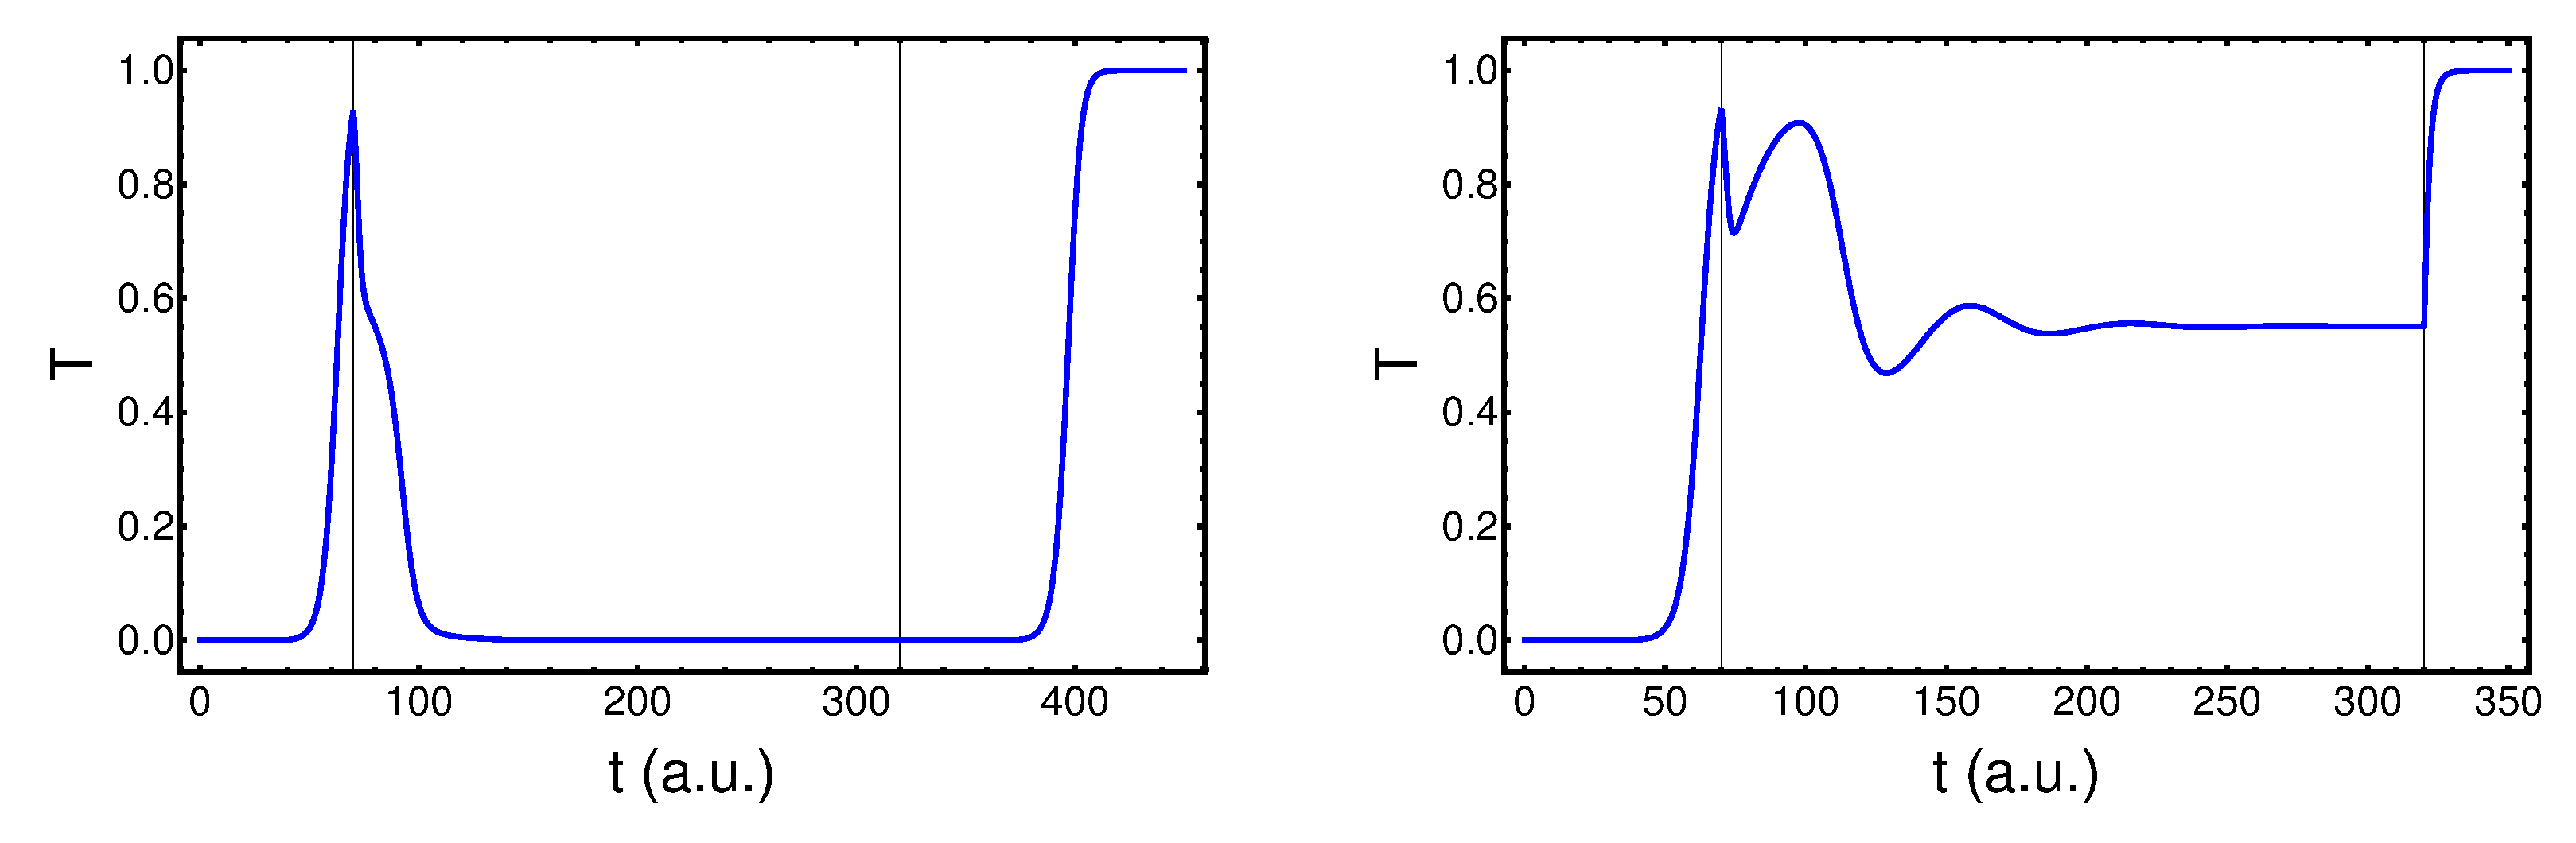
\includegraphics[width=15cm] {esempio-unregolated.pdf}
\caption{Figure of merit for different simulation of eq.s \eqref{eq:sist-semplificato} and \eqref{eq:sist1}.
We simulate an initial development of the leukemia into a healthy steady state 
from one TIC. 
Next, we simulate the therapy with a molecular inhibitor,
like Imatinib, by raising the death rate of leukemic cells
\cite{effetto-imatinib-1, effetto-imatinib-2, effetto-imatinib-3} 
Finally the interruption of the therapy, the black vertical lines represent the start
and stop of the therapy. 
In both figures, the parameters are the same $d_{1,l}=d_{1,h}=0.003$, $d_{2,l}=d_{2,h}=0.005$,
$d_{3,l}=d_{3,h}=0.08$, $a_{1,l}=a_{1,h}=0.65$, $a_{2,l}=a_{2,h}=0.55$, 
$a_{3,l}=a_{3,h}=0.55$, $p_{1,l}=p_{1,h}=1$, $p_{2,l}=p_{2,h}=1.2$,
$p_{3,l}=p_{3,h}=1.3$ and $K_{l}=K_{h}=1.6\times 10^{-10}$. 
The only difference between the two images is that on the
Left, during the therapy $d_{1,l}>(2a_{a,l}-1)p_{1,l}$ we see a monotone 
decay of the tumor burden, and it is only possible to stop the therapy if $m_{1,l}(t)=0$. 
In contrast, the right shows that during the therapy, we have $d_{1,l}=(2a_{a,l}-1)p_{1,l}$, so the tumor size becomes constant after a certain amount of time, 
In this case, it is impossible to interrupt the drug administration without causing a relapse.\\
} 
\label{fig:model1}
\end{figure}

\FloatBarrier

\subsubsection{ Cytokine-dependent leukemic cell lineage}
In this section,
we suppose that 
the CML cells have a cytokine-dependent proliferation,
and we assume that healthy cells and leukemic cells compete for environmental
resources.\\
So, using only two lineages 
one for the healthy cells ($c_{i,h}(t)$) and one for 
the leukemic cells ($c_{i,l}(t)$) ,
we have six first-order differential equations:
\begin{equation}
\begin{array}{ll}
& \frac{dc_{1,h}(t)}{dt}= [(2a_{1,h}s(t)-1)p_{1,h}-d_{1,h}]c_{1,h}(t),\\
& \frac{dc_{2,h}(t)}{dt}=2(1-a_{1,h}s(t))p_{1,h}c_{1,h}(t) +[-d_{2,h}+(2a_{2,h}s(t)-1)p_{2,h}]c_{2,h}(t), \\
& \frac{dc_{3,h}(t)}{dt}=2(1-a_{2,h}s(t))p_{2,h}c_{2,h}(t)-d_{3,h}c_{3,h}(t), \\
& \frac{dc_{1,l}(t)}{dt}= [(2a_{1,l}s(t)-1)p_{1,l}-d_{1,l}]c_{1,l}(t), \\
& \frac{dc_{2,l}(t)}{dt}=2(1-a_{1,l}s(t))p_{1,l}c_{1,l}(t) +[-d_{2,l}+(2a_{2,l}s(t)-1)p_{2,l}]c_{2,l}(t), \\
& \frac{dc_{3,l}(t)}{dt}=2(1-a_{2,l}s(t))p_{2,l}c_{2,l}(t)-d_{3,l}c_{3,l}(t), \\
\end{array}
\label{eq:sist2}
\end{equation}
with $s(t)$ equal to:
\begin{equation}
s(t)=\frac{1}{1+K_hc_{3,h}(t)+K_lc_{3,l}(t)}.
\end{equation}

The system \eqref{eq:sist2}
has three possible equilibriums \cite{stiehl2012mathematical}:
\begin{enumerate}
\item Leukemic steady state,
\item Healthy steady state,
\item Composite steady state.
\end{enumerate}
First of all, we suppose that the parameters of the equations \eqref{eq:sist2} 
are the same before 
and after the treatment. 
Indeed,  if we  discard this hypothesis, it is necessary
to use stochastic differential equations or 
probabilistic
formalisms.\\
Since every patient had developed the leukemia in the past, this could append in two cases 
\begin{enumerate}
\item [a.] We suppose that the BRC-ABL 
mutation gives a proliferation advantage to the leukemic cells. 
Next, the parameters of the patient imply that 
the leukemic steady state is possible and the
healthy steady state is unstable in the direction of $c_{1,l}(t)$, i.e. 
$\frac{a_{1,l}p_{1,l}}{d_{1,l}+p_{1,l}}>\frac{a_{1,h}p_{1,h}}{d_{1,h}+p_{1,h}}$,
$(2a_{1,l}-1)p_{1,l}>d_{1,l}$, $d_{3,l}>0$, 
$\frac{a_{1,l}p_{1,l}}{d_{1,l}+p_{1,l}}>\frac{a_{2,l}p_{2,l}}{d_{2,l}+p_{2,l}}$ and
$\frac{a_{1,l}p_{1,l}}{d_{1,l}+p_{1,l}}>\frac{a_{3,l}p_{3,l}}{d_{3,l}+p_{3,l}}$.


\item [b.] The patient specific parameters admit a steady composite state, i.e. 
$\frac{a_{1,h}p_{1,h}}{d_{1,h}+p_{1,h}}>\frac{a_{2,h}p_{2,h}}{d_{2,h}+p_{2,h}}$,
$\frac{a_{1,h}p_{1,h}}{d_{1,h}+p_{1,h}}>\frac{a_{3,h}p_{3,h}}{d_{3,h}+p_{3,h}}$,
$d_{3,l}>0$, $d_{3,h}>0$ and
$\frac{\frac{d_{1,l}}{p_{1,l}}+1}{2a_{1,l}}=\frac{\frac{d_{1,h}}{p_{1,h}}+1}{2a_{1,h}}$. 
In this case, the leukemia was developed due to the fluctuations in the population 
of the TIC \cite{stiehl2012mathematical} For an example, see figures \ref{fig:fluctuations} and 
\ref{fig:P-fluctuations}.
\end{enumerate}

Next, if we estimate that our patient is an a. type, we are able to have the same possibilities 
of the cytokine-independent model, as seen in figure \ref{fig:stop-pure-l}.\\
In contrast, if the patient lies in the b. case, then the therapy will slowly eradicate the disease. 
However, it is possible to stop the therapy before, as the interruption will leave
the patient in another composite state, defining $\alpha:=(p_{1,l}d_{3,l}-p_{1,h}d_{3,h})(d_{3,h}-d_{3,l})$, we have three different possibilities 
\cite{stiehl2012mathematical}:
\begin{itemize}
\item $\alpha<0$ the system is stable in the sense that it asymptotically approaches the center manifold if it starts in
the neighborhood of it. This condition implies $p_{1,l}d_{3,l}>p_{1,h}d_{d_{3,h}} $
and $d_{3,h}>d_{3,l}$ or $p_{1,l}d_{3,l}<p_{1,h}d_{d_{3,h}} $
and $d_{3,h}<d_{3,l}$.
\item $\alpha=0$ if and only if either $p_{1,l}d_{3,l}=p_{1,h}d_{3,h}$ or $d_{3,l}=d_{3,h}$.
In these cases, the system is stable in the sense that it will asymptotically approach the center manifold
if it starts in the neighborhood of it,
if \item $\alpha>0$ and $K_{l}c_{3,h}(t)$ is small enough, then the system would be stable 
if it starts in the neighborhood of a center manifold.
\end{itemize}



\begin{figure}
\centering
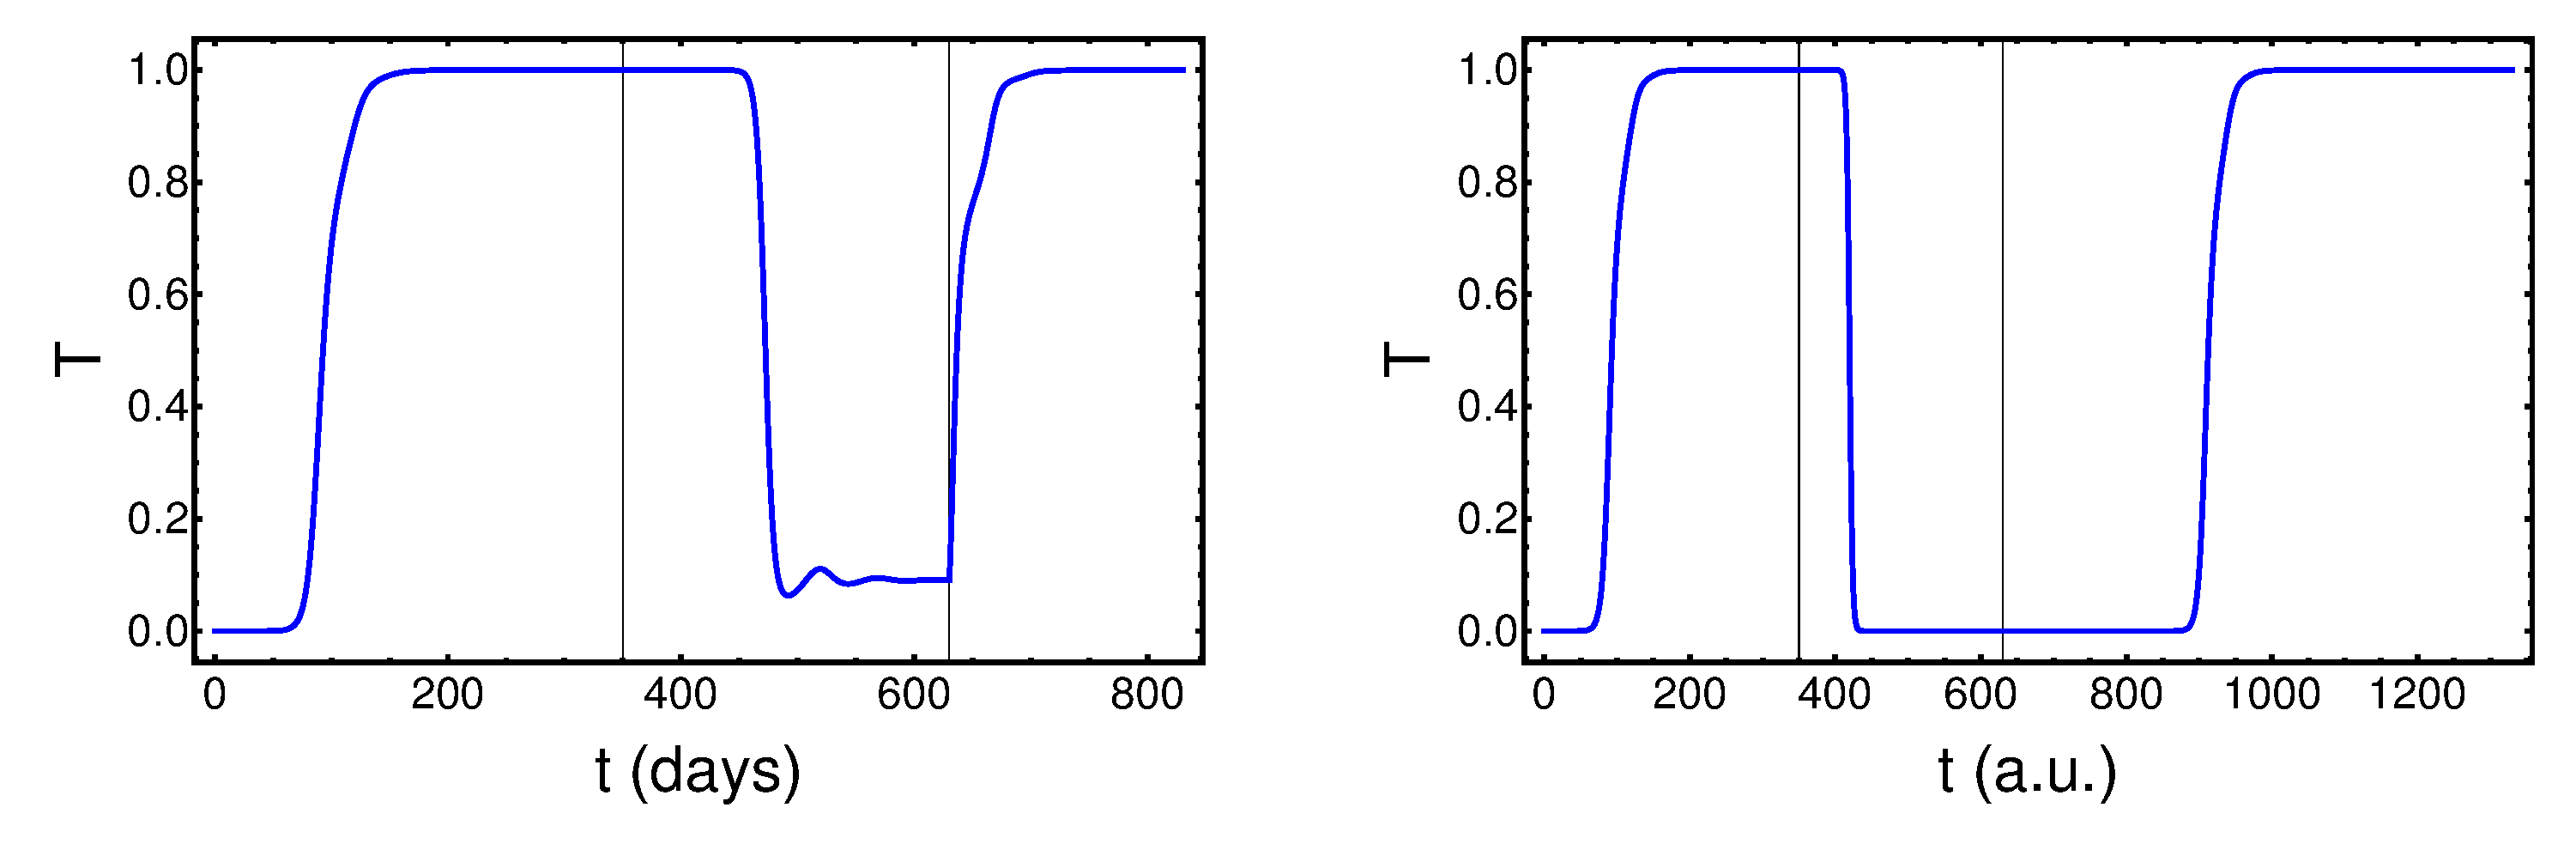
\includegraphics[width=13cm] {stop-terapia-caso-regolated.pdf}
\caption{Figure of merit of the therapy and the stop, obtained by
solving eq.s \eqref{eq:sist2}. We choose of parameters in order to have a 
composite steady state: 
$d_{1,l}=d_{1,h}=0.003$, $d_{2,l}=d_{2,h}=0.005$,
$d_{3,l}=d_{3,h}=0.08$, $a_{1,l}=a_{1,h}=0.65$, $a_{2,l}=a_{2,h}=0.55$, 
$a_{3,l}=a_{3,h}=0.55$, $p_{1,l}>p_{1,h}=1$, $p_{2,l}=p_{2,h}=1.2$ and
$p_{3,l}=p_{3,h}=1.3$, $K_{l}=K_{h}=1.6\times 10^{-10}$.\\
In this case, the left shows the effects of the drugs that lead to a composite state, while
the right is that of a pure healthy state.\\
In the first case, it is not possible to stop the therapy. In the second,
this is possible only when the tumor is eradicated.}
\label{fig:stop-pure-l}
\end{figure}
\begin{figure}
\centering
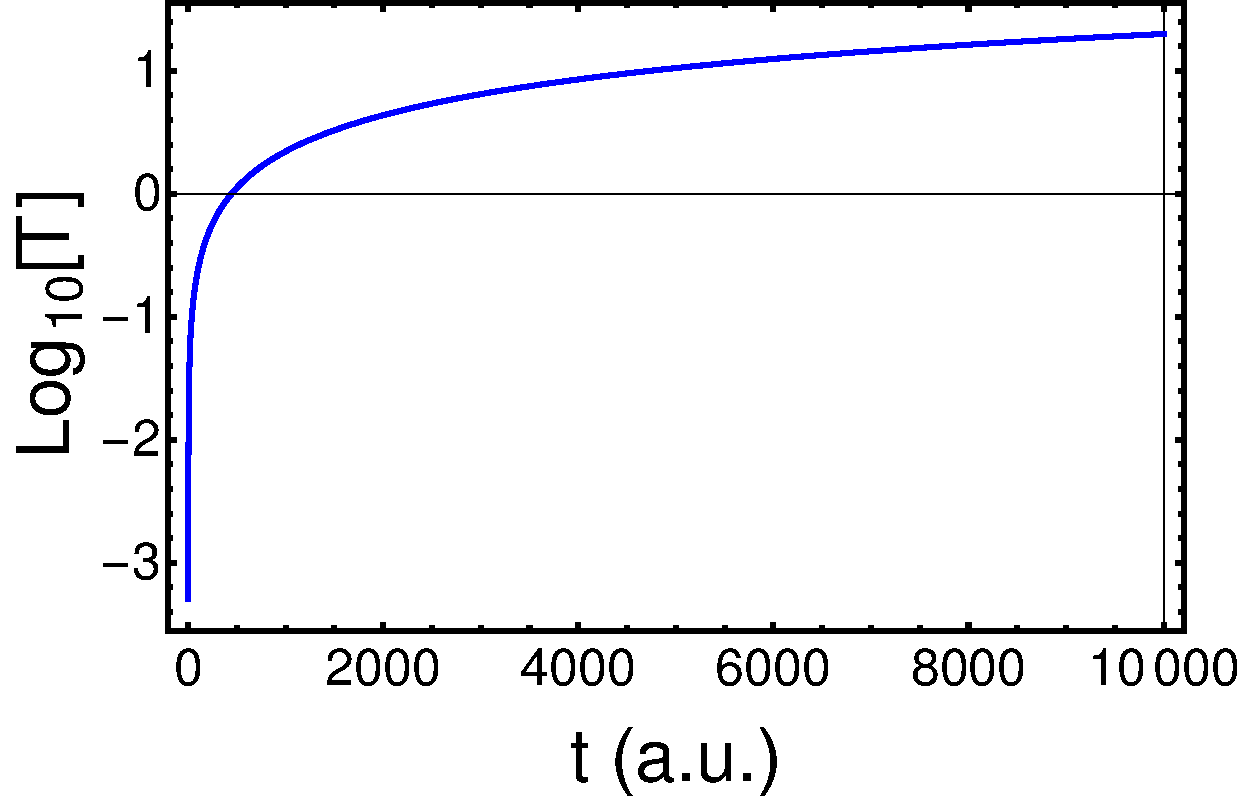
\includegraphics[width=10cm ]{blast-fluct.pdf}
\caption{Figure of merit obtained solving eq.s \eqref{eq:sist2}.
We added $10^4$ TIC to a healthy steady state, and we chose the parameters required to have a 
composite steady state: 
$d_{1,l}=d_{1,h}=0.003$, $d_{2,l}=d_{2,h}=0.005$,
$d_{3,l}=d_{3,h}=0.08$, $a_{1,l}=a_{1,h}=0.65$, $a_{2,l}=a_{2,h}=0.55$, 
$a_{3,l}=a_{3,h}=0.55$, $p_{1,l}=p_{1,h}=1$, $p_{2,l}=p_{2,h}=1.2$ and
$p_{3,l}=p_{3,h}=1.3$, $K_{l}=K_{h}=1.6\times 10^{-10}$.\\
In this case, the we add random noise $x\in[-10^3,10^3]$ to $c_{1,l}(t)$,
Note that leukemia would not be able to develop without the fluctuations, 
but the fluctuations does not inherently imply the presence of the disease. }
\label{fig:fluctuations}
\end{figure}

\begin{figure}
\centering
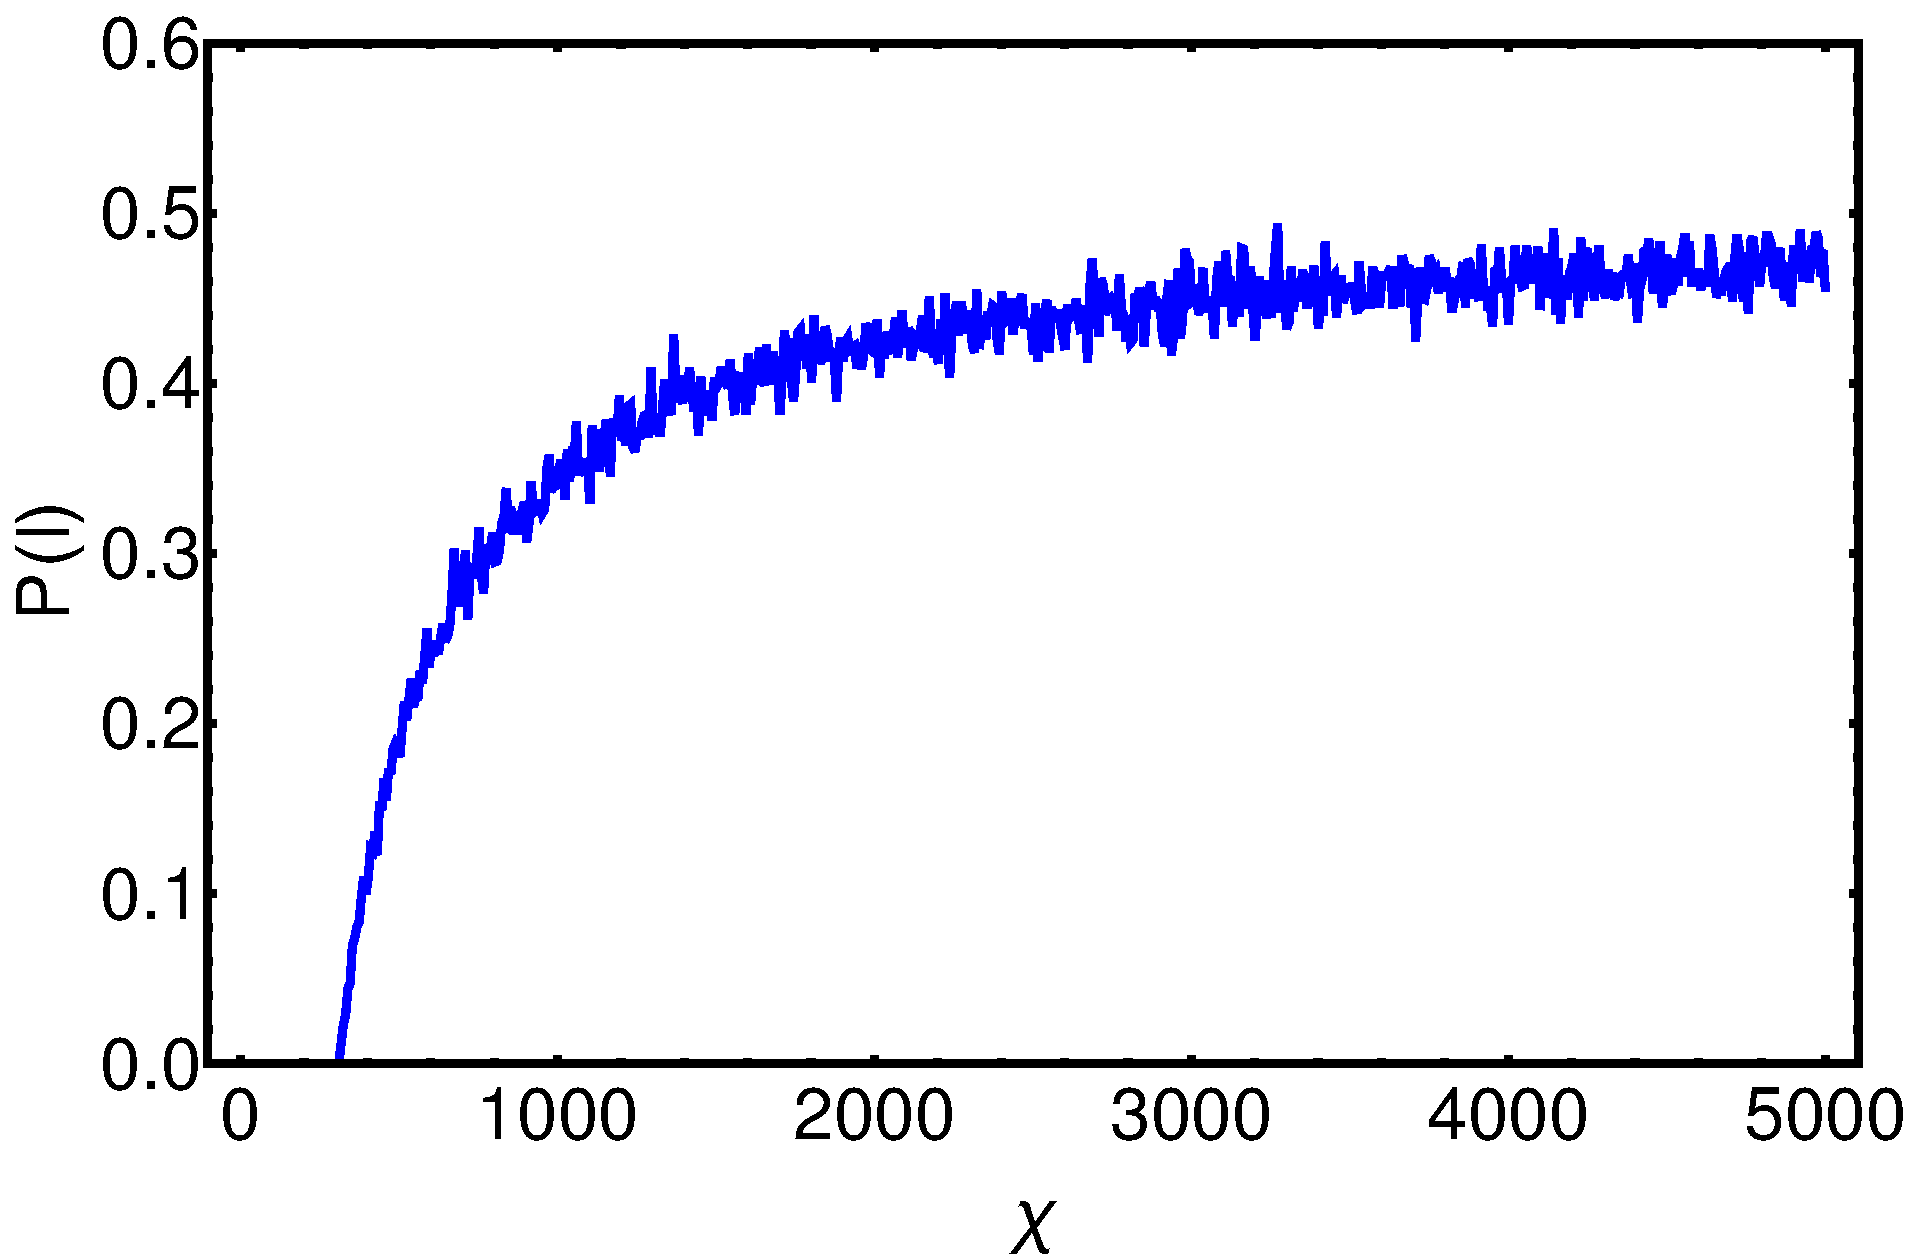
\includegraphics[width=10cm] {leucemia-e-fluttuazioni.pdf}
\caption{Probability to develop a leukemia $P(l)$ with $T\geq0.01$ after
$5000$ units of time in function of the range of a stochastic noise, $x\in[-\chi,\chi]$,
added to $c_{1,l}(t)$ or $c_{1,h}(t)$. This probability was evaluated with $2000$ repetitions for any value of $\chi$.
We started from a composite equilibrium with $10^4$ TIC, where approximately $ 100\%$ of the
cells are healthy;
the parameters of this simulation are: 
$d_{1,l}=d_{1,h}=0.003$, $d_{2,l}=d_{2,h}=0.005$,
$d_{3,l}=d_{3,h}=0.08$, $a_{1,l}=a_{1,h}=0.65$, $a_{2,l}=a_{2,h}=0.55$, 
$a_{3,l}=a_{3,h}=0.55$, $p_{1,l}=p_{1,h}=1$, $p_{2,l}=p_{2,h}=1.2$ and
$p_{3,l}=p_{3,h}=1.3$, $K_{l}=K_{h}=1.6\times 10^{-10}$.\\
}
\label{fig:P-fluctuations}
\end{figure}


\begin{figure}
\centering
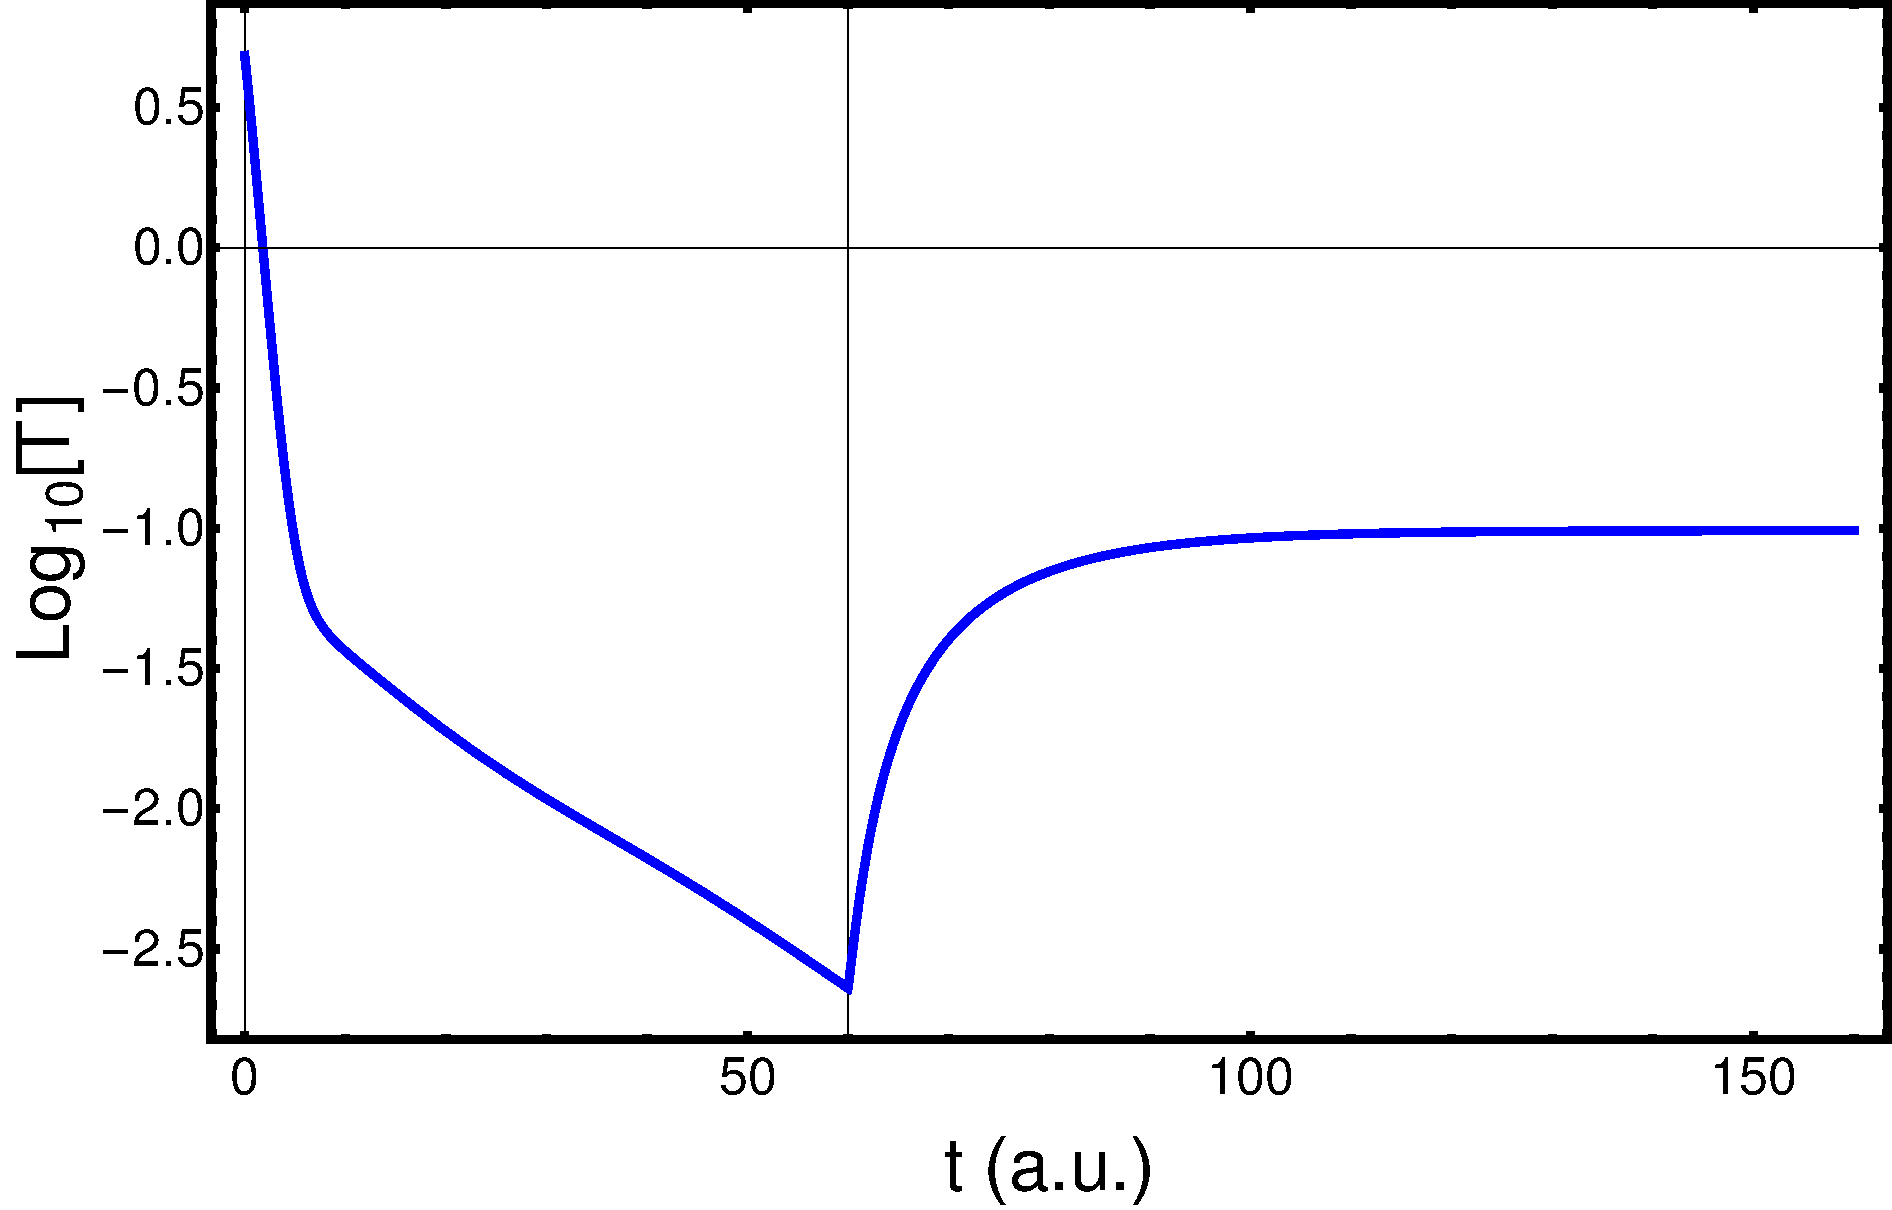
\includegraphics[width=10cm ]{stop-composite.pdf}
\caption{Figure of merit  of the therapy and the stop, obtained by
solving eq.s \eqref{eq:sist2}.
We choose the parameters in order to have a 
composite steady state: 
$d_{1,l}=d_{1,h}=0.003$, $d_{2,l}=d_{2,h}=0.005$,
$d_{3,l}=d_{3,h}=0.08$, $a_{1,l}=a_{1,h}=0.65$,  $a_{2,l}=a_{2,h}=0.55$,  
$a_{3,l}=a_{3,h}=0.55$, $p_{1,l}=p_{1,h}=1$, $p_{2,l}=p_{2,h}=1.2$ and
$p_{3,l}=p_{3,h}=1.3$, $K_{l}=K_{h}=K_{sh}=K_{lh}=1.6\times 10^{-10}$.\\
In this case we can see the typical decay with two slopes \cite{michor2005}, 
this double decay it is due to a different slope of decay between HSC and PC.
After the stop of the therapy, the vertical black line,
 the systems reaches a new composite steady state with less leukemic cells.}
\label{fig:stop-composite}
\end{figure}



\FloatBarrier
\subsection{Pharmacodynamics and Pharmacokinetiks}
In the previous section, we simplified the action 
of the molecular inhibitor, as an increasing of the death rate of not-TD CML cell lineage.
However, works like \cite{ishida2016pharmacokinetics, yoshitsugu2012markov}
suggest that the anti-leukemic 
activity of the treatment was time-dependent. 
As such, to better design the effects of the dosage, we model the concentration in the blood vs
time as a Lasota
\cite{wazewska1976matematyczne} function:
\begin{equation}
C(t)=A t e^{-Bt}
\label{eq:lasota}
\end{equation}
where $A$ and $B$ are two real and positive constants.\\
Then, we model the effect of the concentration of Imatinib as an increment 
of the rate of death, which is modulated by a sigmodean-like function:
\begin{equation}
d_{i,l}(t)= \left(1-\frac{2(1- d_{i,l}^0)}{1-CExp(-Ft)} \right)
\label{eq:sigmodean}
\end{equation}
where $C$ and $F$ are two real and positive constants
and $d_{i,l}^0$ are the values of the death rate of the first
two compartments of leukemic cells without treatment. Note that this function
was chosen in order to obtain $d_{i,l}(t)=d_{i,l}^0$ when $C(t)=0$ and $d_{i,l}(t)=1$
when the concentration reached its maximum.\\
An example of the behavior of the equations \eqref{eq:lasota} and \eqref{eq:sigmodean} 
is shown in figure \ref{fig:dose}.\\
It is important to point out that
since we integrated the system \ref{eq:sist2} for a long-time, with respect
to the period of the function $C(t)$,
it would be the same to consider any $L^1(\mathbb{R},dt)$ 
function respective to \eqref{eq:sigmodean},
with the only relevant quantity being the value of the integral
$N= \int_{t_0}^{t_1} d_{i,l}(t) dt$.
Next, if we used a constant with the same numerical value 
(i.e. $ \frac{\int_{t_0}^{t_1}d_{i,l}(t)}{(t_1-t_0)}=d_{i,l} $) 
of the integral, 
the numerical solution of \eqref{eq:sist2} will be the same.
From the mathematical point of view,
this approximation holds true only if the time lapse under study (integration) is 
slightly bigger with respect to the periodicity of the 
administration of the drugs,
Instead from the biological point of view, 
this would reflect  Haber's rule \cite{miller2000haber}
$cost.= C\times t$, where $C$ is the concentration of a substance 
and $t$ is the length of time in which it is administered.\\


\begin{figure}
\centering
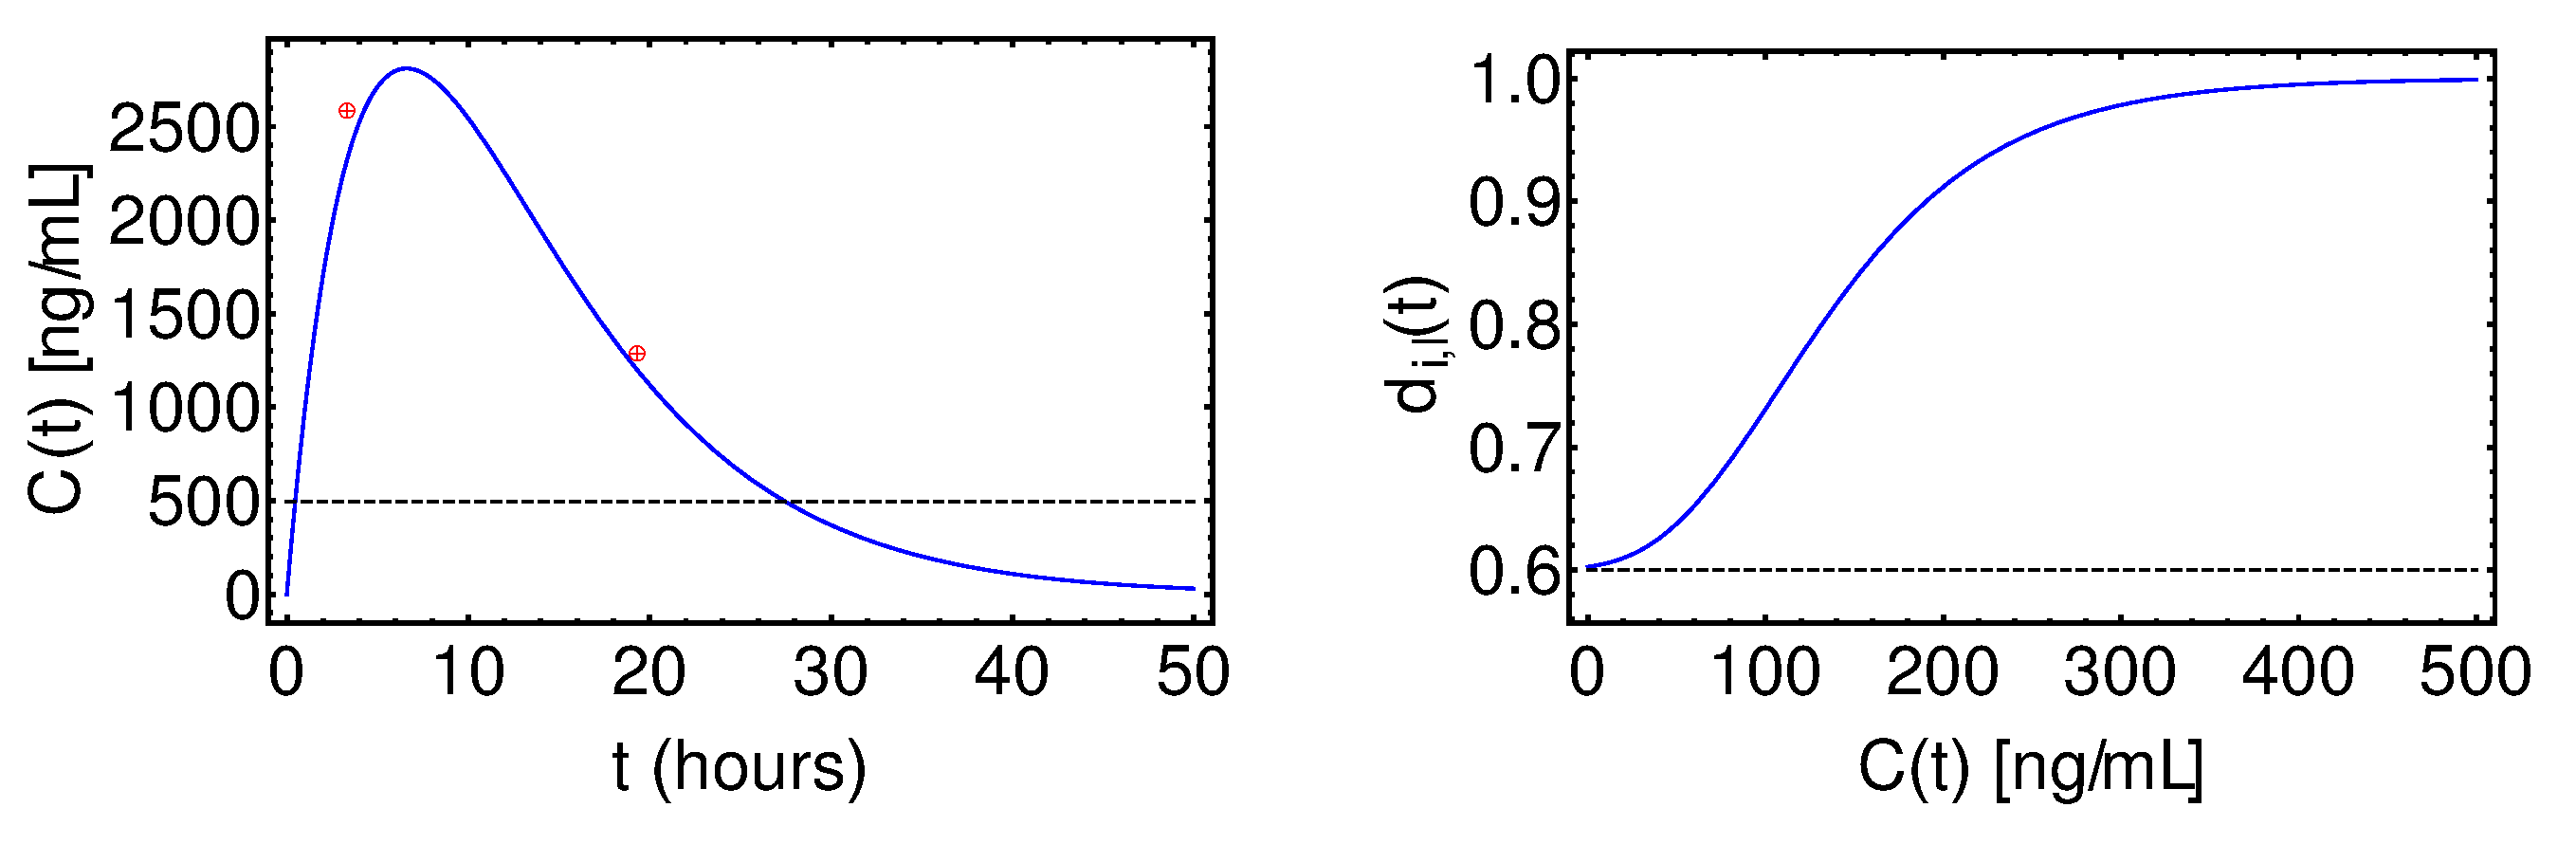
\includegraphics[width=14cm] {farmaco-dy.pdf}
\caption{ On the left is the simulation of the pharmacokinetics of 400 mg Imatinib administration,
as stated in \cite{ishida2016pharmacokinetics}, and on the right are the effects of the therapy on the death rate of leukemic cells,
the dashed red line is $d_{i,l}^0=0.60$. The parameters of equations 
\eqref{eq:sigmodean} and \eqref{eq:lasota} are $A=407$, $B=1$, $C=1$ and $F=1$}
\label{fig:dose} 
\end{figure}


\FloatBarrier

\section{Tuning of the parameters}
The model presented in the preceding section is thus able to give some predictive 
information regarding the course of the disease in a patient and to 
understand if the therapy can be stopped.
However, this ability is limited by three factors 
\begin{itemize}
\item The quantity studied in the experimental works (e.g. \cite{michor2005, olshen2014dynamics}) 
is the molecular response (MR). 
Thus, it is an open question as to whether this quantity will always correlate with the 
cell count of tumor and if other 
measurement techniques would be better 
\cite{rainero2018gdna, experiment-affidabile-1, experiment-affidabile-2, experiment-affidabile-3,
experiment-affidabile-4, latham2016bcr}.
\item The experimental data is a relative 
information.
Instead, the model requires
quantitative information 
regarding the number of cells in a class.
\item Discussion on the number of ensembles in a lineage with respect to the parameters. 
\end{itemize}
To overcome this problems, we make the following assumptions.
Regarding the first one, we suppose that the proportionality between MR and cell counts holds.
Indeed, only further experiments can solve any further problems with this supposition.\\
The second problem is trickier, 
as if one tries to make a fit 
between the FOM and the values,
as reported in the data, he will struggle with the fact that it is necessary to make
a non-trivial guess 
on the initial conditions, 
and consequently, the value of the parameters that he will obtain would be dependent on 
this initial guess. 
Furthermore, by minimizing some notion of distance 
one will find the FOM closer to the data, and this 
FOM $F(\mathbb{A},\mathbf{x}_0)$ 
would be completely described by the collection of its parameters 
$\mathbb{A}$ and initial condition $\mathbf{x}_0$.
However, a couple of
$(\mathbb{A}',\mathbf{x}_0')$ will exist such that
$F(\mathbb{A},\mathbf{x}_0)=F(\mathbb{A}',\mathbf{x}'_0)$.
For these reasons, every result obtained with this model 
should be treated with attention. Since every estimation of the parameters
depends on an arbitrary guess, the values of the parameters that is
obtained through a data analysis will be one of the possible
solutions with the same FOM.
As such, the focus during data analysis
should be to address the behavior, 
not the absolute values of the results.
This will hold true till will be accessible the information about
the cell count in particular at the start of the therapy,
and it is only through this condition will the tuning of the
parameters in order to be consistent with the international
scale for MR \cite{white2013establishment}.\\ 
First of all, we are going to reduce the attention 
on the biologically 
relevant range of parameters \cite{stiehl2012mathematical}:
\begin{equation}
\begin{array}{lll}
\frac{1}{2}<\bar{s}<1, & 0\leq K_{l}\bar{c}_{3,l}\leq (2a_{1,l}), & 0\leq K_{h}\bar{c}_{3,h}\leq (2a_{1,h}), \\ 
\end{array}
\end{equation}



then, supposing that the relevant experimental data is not the absolute value of 
the MR, but it variation (the behavior), we made the data analysis in the following way:
We gave  $n$ data for a follow up, while
$O(t_i)$ for $i=1,\dots n$ and the FOM $T(t_i, \mathbb{A})$ 
 was obtained by numerically solving the system at $t_i$ for a certain collection 
of parameters $\mathbb{A} $, 
Next, we defined a matrix of $F_K$, which elements were given by:
\begin{equation}
F_{K,ij}=(1-\delta_{ij})\frac{K_i-K_j}{t_i-t_j}
\end{equation}
where $\delta_{ij}$ is the Kronecker delta and $K_{i}=O(t_i), \quad T(t_i, \mathbb{A})$.\\
This symmetric matrix contains the value of all the incremental ratios contained in the experimental data.
Finally, we minimized the 2-norm distance between $F_{O}$ and $ F_{T}$, i.e.:
\begin{equation}
D=\sum_{i=1}^n\sum_{j=1}^n\sqrt{(|F_{O,ij}|^2- |F_{T,ij}|^2)}.
\end{equation}
We chose to study this quantity as minimizing the differences between the theoretical
and observed incremental ratio between the pair of neighbor points will promote local trends 
from the derivatives.\\
The minimization was performed by a random search algorithm that worked in the following way:
\begin{enumerate}
\item Make a random initial guess on the parameters $\mathbb{A}$ 
\item Make a random step in the parameters space $\mathbb{A}\longrightarrow\mathbb{A}'$
\item Solve the system \eqref{eq:sist2} using $\mathbb{A}'$
\item Evaluate $D$
\item If $D$ evaluated with $\mathbb{A}'$ is lesser than $D$ evaluated using $\mathbb{A}$,
then go back to 2 and use $\mathbb{A}'$ as an initial guess, or else go back to 2. 
\end{enumerate}
If $\mathbb{A}$ and $\mathbb{A}'$ had the same $D$, we chose the case that minimized:
\begin{equation}
\chi^2=1-\sum_{i}^n\frac{O(t_i)-T(t_i)}{T(t_i)}
\end{equation}

In order to have a more robust procedure, we added a super iteration (SI) on the initial guess. 
Both random seeds were obtained using the Sobol sequence \cite{bergstra2012random}.
An example of the analysis of a patient of \cite{michor2005} 
is shown in figure \ref{fig:data-analysis}.
In this case, due to the time-span of 
the follow up and the periodic dosage of the molecular inhibitor
we modeled the Pharmacodynamics that we used with a constant reduction estimated in \cite{michor2005}.
\begin{figure}
\centering
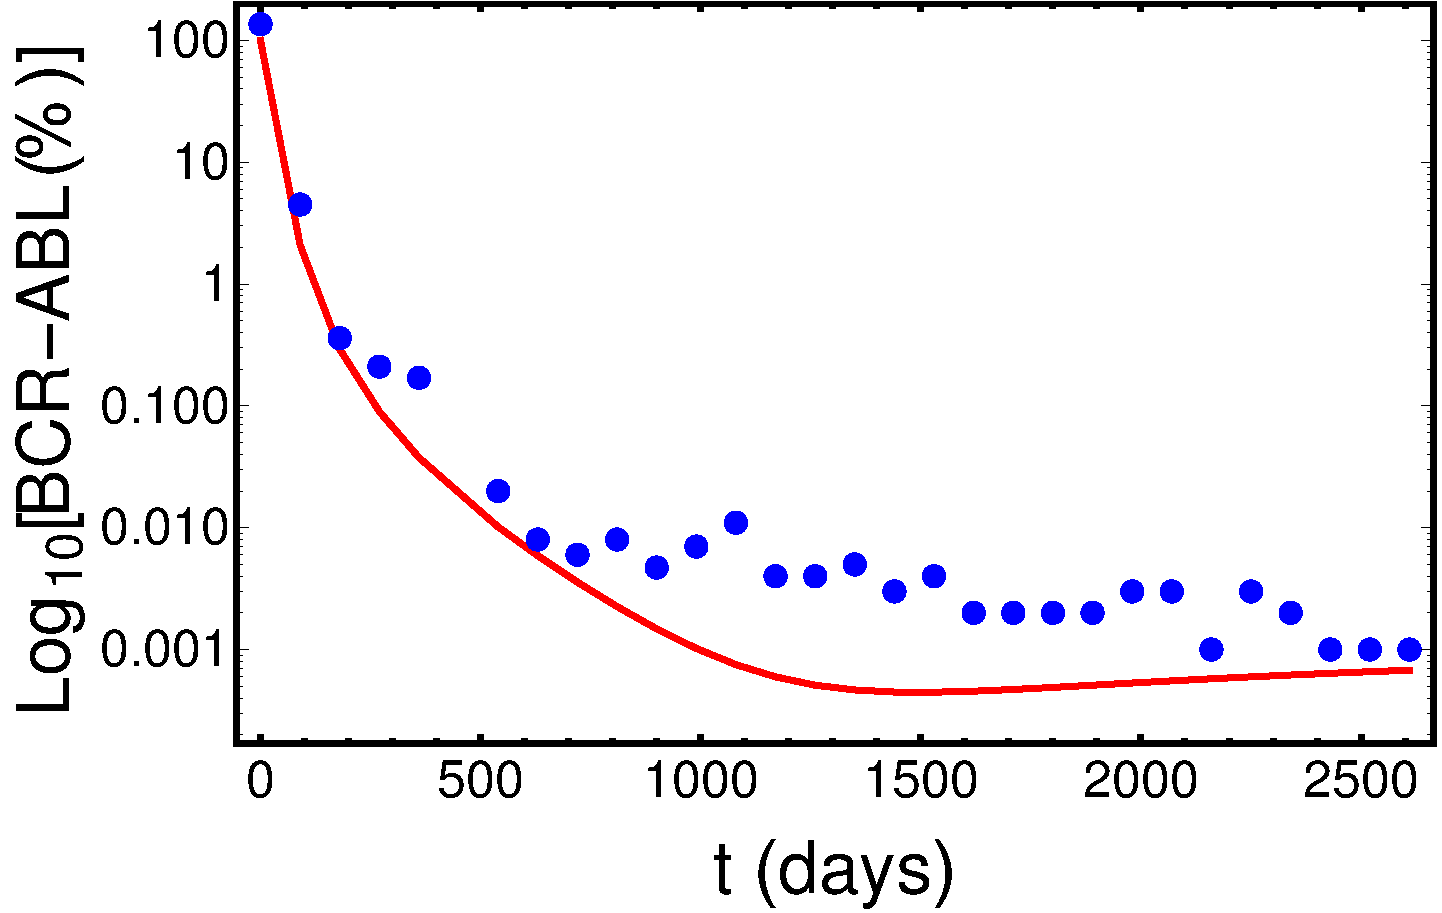
\includegraphics[width=9cm ]
{analisi-paziente1.pdf}
\caption{The blue points are data of a follow up from \cite{michor2005}, and the red solid line is the best fit obtained using the procedure described in this work, with a 500 SI and 1100 iteration of 
the algorithm.
In this example, we fixed the initial condition, and fixed the death rate $d_{i,k}$ from the work \cite{michor2005} then $d_{i,l}=d_{i,h}$ for $i=1,2,3,4$ with $d_1=0.003$ per day, $d_2=0.008$ per day,
$d_3=0.05$ per day, and $d_4=1$ per day,
the probability of self-renewal was fixed $ a_{i,l}=a_{i,h}$ for $i=1,2,3,4$ $a_1=0.7$, $a_2=0.65$, $a_{3}=0.55$ and $a_{4}=0.55$, $K=1.3 \times 10^{-7}$. Finally, we suppose that during the treatment 
$p_{1,h}=2p_{1,l}/100$, $p_{2,h}=2p_{2,l}/750$ and $p_{3,h}=p_{3,l}$. The obtained values were $p_{1h}=6.986$ per day, $p_{2,h}=0.0137$ per day, $p_{3h}=2.014$ per day and
$\lambda= 2.2 \times 10^{-8}$ per day. The results of the two tests were $\chi=0.990$ and $D=2.602$. Note that the final state was reached from an analysis of the eigenvalue of the Jacobian results
unstable, in fact if the simulation is performed for later times, it reached a stable state higher than the final state and this stable state 
was different from the minimum of $T$. The minimum was reached just after the first 3-fold decay. 
This peculiar behavior was caused by the signal, as it had a big increase just after this decline.}
\label{fig:data-analysis}
\end{figure}
\FloatBarrier
\section{Optimization of the therapy}
A mathematical model of the disease and its therapy gave the possibility of making
a \textit{in silico} optimization of the therapy 
\cite{tannenbaum2018control, nanda2007optimal}. 
With regarding to the optimization, we mean 
balancing certain therapy costs against performance. For example,
the cost
of the therapy could be an economic cost 
\cite{experts2013price, jabbour2017evaluation, himmelstein2009medical, chen2017journey, gomez2017insights} 
or toxicity of the therapy 
\cite{zhu2014clinical, hu2012mechanistic, breccia2008differences, cohen2002approval}
and 
the reduction in the tumor burden of a patient could be used as the performance. 
Such a kind of study could be very useful,
in particular for the CML, 
as the treatment is very expensive
\cite{experts2013price, jabbour2017evaluation, chen2017journey} such
that it could limit the patient’s access to therapy 
\cite{gomez2017insights, himmelstein2009medical} and 
lowering the prices of therapy will
allow more patients to afford it and 
maintain a long-term health care policy \cite{fojo2009much}. It is also possible that
sub-clonal resistant mutation 
could arise and would make it necessary to manage
the switch to a new molecular therapy \cite{cortes2016evaluating} 
In this case, we suppose that 
the therapy fails in eradicating the disease (then it is life-long therapy)
and a low dosage could be useful 
in minimize the toxicity of the therapy \cite{faber2016lower}.\\
To perform this optimization, we will use the control theory, in particular we will 
use an open loop control. A key aspect of this theory is the cost.
As such, we defined the following cost function:
\begin{equation}
\mathbb{J}(t):=\int_{t_{in}}^{t_{fin}}\left(\mathbf{A}(d(t))+\mathbf{B}(d(t))+\mathbf{C}(T(t))
+\mathbf{D}(R(t)) \right) dt
\end{equation}
where $t_{in}$ and $t_{fin}$ are initial and final time of the interval under study,
$\mathbf{A}(d(t))$ represents the economic cost of the therapy,
$\mathbf{B}(d(t))$ represents the cumulative toxicity of the therapy,
$\mathbf{C}(T(t))$ represents the 
cost in quality of life due to the burden of cancer during the therapy, and 
$\mathbf{D}(R(t))$ is the cost of the risk of developing a resistant mutation.\\
Obviously, we need an explicit formula for every elements of the cost.
For the economic cost, we imposed that it is  linear respect to 
the dose $\mathbf{A}(d(t))=Ad(t)$, As such, it can be argued that if the cost was about
$120,000\$$ year at 400 mg per day \cite{chen2017journey}, the cost for 1 mg
of Imatinib was about $0,8333\$$, thus fixing the value of $A$.\\
Regarding the cumulative toxicity of the drugs,
Imatinib could cause a grade 3/4 (Common Terminology Criteria for Adverse Events (CTCAE)
V5.0) Adverse Events (AE), and dose-limiting toxicity was not
observed \cite{cohen2002approval}. However, only to a small fraction of AE 
was attributed to Imatinib \cite{cohen2002approval}. Then, 
for this case, we suppose that the long-term
adverse effects are negligible, and they are quite acceptable \cite{mughal2010principal}.
i.e. $\mathbf{B}(d(t))=0$. Finally, since an accidental Imatinib
over-dosage could cause reversible bilirubin 
and transaminase elevation \cite{cohen2002approval}
we bound the maximum dose at $900$ mg per day.\\ 
During the therapy, we saw a great improvement of the quality of life
after the first 3-fold decay, i.e. when $T(t)<0.0001$ (cit.). Under this threshold
no big improvements are observed. To model this behavior, we used the following function:
\begin{equation}
\mathbf{C}(T(t))=C_1e^{C_2(T(t)-T_0)}, 
\end{equation}
where $C_i$ for $i=1,2$ are two real constants. This function gives the exponential cost
if $T(t)>T_0$. However, as we will see below, $C_1$ could be set to 0.\\
Finally, we need to study the function that represents the risk associated to developing a 
resistant mutation $\mathbf{D}(R(t))$. 
We suppose that every CSC, when proliferating, 
has a certain probability $r$ to develop a resistant mutation. In such cases, it would
generate a resistant CSC.
Thus, we estimate the risk of having a resistant mutation as the number of resistant cancer cells
in respect to the total number of cells of the system, and to evaluate this quantity, we use a third
cell lineage $c_{i,r}(t)$ (servono test per capire se \'e meglio cos\'i oppure conviene
porre una quantit\'a direttamente
proporzionale alle CSC, la seconda dovrebbe essere migliore in realt\'a).

\printbibliography
\end{document}
